The selection into preschool, as well as the selection into a particular type of preschool, might be determined by social, demographic, and economic characteristics of the family. We begin by presenting a linear probability model to predict the probability of selecting into (i) preschool or (ii) infant-toddler care and preschool based on background characteristics.

For an individual $i$, let $V_i$ indicate selection into preschool and $B_i$ indicate selection into both preschool and infant-toddler care.\footnote{There are too few people who selected only into infant-toddler care to consider that option as well.} Given a vector of binary characteristics $\mathbf{X}_i$, we perform the following regressions by city and cohort:

\begin{align}
	V_i &= \alpha_0 + \mathbf{X}_i\bm{\alpha} + \upsilon_i \label{eq:lpm-v} \\
	B_i &= \gamma_0 + \mathbf{X}_i\bm{\gamma} + \epsilon_i. \label{eq:lpm-b}
\end{align}

We combine Italian and non-Italian children into one cohort, but include an indicator for migrant in $\mathbf{X}$. Tables~\ref{tab:lpmRE} through \ref{tab:lpmPD} give the estimates of this model. These estimates reveal the percentage a particular characteristic contributes to the probability of enrolling in preschool (and infant-toddler care). 

\begin{sidewaystable}[H]
	\caption{Linear Probability Model, Reggio Emilia}\label{tab:lpmRE}
	\centering
	\footnotesize
		\begin{tabular}{lcccccccccc} \toprule
& \mc{2}{c}{Children} & \mc{2}{c}{Adolescents} & \mc{2}{c}{Adults 30s} &  \mc{2}{c}{Adults 40s} & \mc{2}{c}{Adults 50s} \\
\cmidrule(lr){2-3} \cmidrule(lr){4-5} \cmidrule(lr){6-7} \cmidrule(lr){8-9} \cmidrule(lr){10-11}
 & Preschool & Both & Preschool & Both & Preschool & Both & Preschool & Both & Preschool & Both \\ \midrule
Mother Worked Full Time & 0.033** & 0.367*** & 0.130*** & 0.635*** & 0.298*** & 0.088 & 0.486*** & 0.168*** & 0.240*** &  \\
 & (0.016) & (0.063) & (0.026) & (0.086) & (0.053) & (0.062) & (0.054) & (0.050) & (0.063) &  \\
Mother Worked Part Time & 0.041** & 0.392*** & 0.110*** & 0.483*** & 0.338*** & 0.214** & 0.443*** & 0.042 & 0.094 &  \\
 & (0.018) & (0.067) & (0.028) & (0.093) & (0.081) & (0.094) & (0.061) & (0.057) & (0.075) &  \\
Two Siblings or More & -0.019 & -0.039 & -0.004 & -0.066 & -0.075 & -0.083 & -0.065 & -0.095* & -0.106 &  \\
 & (0.015) & (0.056) & (0.019) & (0.064) & (0.055) & (0.063) & (0.052) & (0.048) & (0.070) &  \\
One Sibling or More & 0.010 & 0.091* & 0.020 & 0.029 & 0.113* & 0.053 & -0.068 & 0.011 & 0.181 &  \\
 & (0.015) & (0.055) & (0.021) & (0.070) & (0.062) & (0.072) & (0.062) & (0.058) & (0.115) &  \\
Mother Born in Province & -0.008 & -0.131** & -0.034* & 0.028 & 0.006 & -0.102 & 0.219*** & -0.030 & 0.103 &  \\
 & (0.015) & (0.059) & (0.019) & (0.063) & (0.067) & (0.077) & (0.058) & (0.054) & (0.074) &  \\
Mother Max. Edu.: Middle Sch. & 0.029 & -0.038 & 0.016 & 0.142 & 0.040 & 0.285 & 0.219 & 0.287 & 0.664** &  \\
 & (0.029) & (0.110) & (0.037) & (0.121) & (0.404) & (0.467) & (0.213) & (0.197) & (0.326) &  \\
Mother Max. Edu.: High Sch. & 0.014 & 0.085 & -0.020 & 0.058 & -0.053 & 0.155 & 0.099 & 0.241 & 0.647* &  \\
 & (0.016) & (0.059) & (0.025) & (0.082) & (0.417) & (0.481) & (0.206) & (0.191) & (0.335) &  \\
Mother Max. Edu.: University & 0.014 & 0.196*** & 0.012 & 0.059 & -0.194 & 0.120 & 0.052 & 0.267 & 0.523 &  \\
 & (0.019) & (0.074) & (0.028) & (0.093) & (0.419) & (0.484) & (0.205) & (0.190) & (0.342) &  \\
Father Born in Province & -0.007 & -0.085 & 0.005 & -0.034 & 0.011 & 0.038 & 0.001 & 0.042 & -0.021 &  \\
 & (0.015) & (0.059) & (0.018) & (0.060) & (0.071) & (0.082) & (0.055) & (0.051) & (0.080) &  \\
Father Max. Edu.: Middle Sch. & -0.038 & 0.098 & 0.025 & -0.058 & 0.058 & -0.745 & -0.028 & -0.048 & -0.235 &  \\
 & (0.028) & (0.106) & (0.034) & (0.114) & (0.416) & (0.480) & (0.195) & (0.181) & (0.324) & \\
Father Max. Edu.: High Sch. & -0.003 & 0.030 & 0.007 & 0.041 & -0.054 & -0.713 & 0.000 & -0.251 & -0.502 &  \\
 & (0.015) & (0.056) & (0.021) & (0.069) & (0.381) & (0.440) & (0.188) & (0.174) & (0.337) &  \\
Father Max. Edu.: University & 0.006 & 0.082 & -0.046* & 0.153* & -0.026 & -0.636 & -0.045 & -0.257 & -0.531 &  \\
 & (0.019) & (0.072) & (0.027) & (0.088) & (0.383) & (0.442) & (0.188) & (0.174) & (0.343) &  \\
Caregiver is Religious & 0.060*** & -0.025 & 0.003 & -0.038 & -0.111** & -0.100* & -0.046 & -0.022 & 0.005 & \\
 & (0.017) & (0.063) & (0.020) & (0.066) & (0.048) & (0.055) & (0.045) & (0.042) & (0.072) &  \\
H. Income Above Median & -0.011 & -0.084* & 0.015 & -0.064 &  &  &  &  &  &  \\
 & (0.013) & (0.048) & (0.017) & (0.058) &  &  &  &  &  &  \\
Caregiver Politics: Right of the Median & -0.002 & -0.046 & -0.011 & 0.065 &  &  &  &  &  &  \\
 & (0.014) & (0.052) & (0.017) & (0.056) &  &  &  &  &  &  \\
Non-Italian Child & -0.036 & -0.092 &  &  &  &  &  &  &  &  \\
 & (0.027) & (0.102) &  &  &  &  &  &  &  &  \\
Low Birthweight & 0.004 & -0.067 & -0.015 & -0.054 &  &  &  &  &  &  \\
 & (0.028) & (0.106) & (0.041) & (0.136) &  &  &  &  &  &  \\
Premature Birth & 0.002 & 0.224** & 0.002 & -0.010 &  &  &  &  &  &  \\
 & (0.027) & (0.101) & (0.038) & (0.127) &  &  &  &  &  &  \\
Constant & 0.912*** & 0.315*** & 0.888*** & -0.010 & 0.718 & 0.787 & 0.231 & 0.045 & -0.217 &  \\
 & (0.029) & (0.110) & (0.034) & (0.113) & (0.567) & (0.655) & (0.151) & (0.140) & (0.370) &  \\
\midrule
$N$ enrolled & 415 & 242 & 293 & 170 & 223 & 69 & 205 & 41 & 53 & 0 \\
$N$ not enrolled & 6 & 179 & 7 & 130 & 57 & 211 & 80 & 244 & 147 & 200 \\
Total $N$ & 421 & 421 & 300 & 300 & 280 & 280 & 285 & 285 & 200 & 200 \\
$R^2$ & 0.079 & 0.230 & 0.236 & 0.223 & 0.206 & 0.075 & 0.419 & 0.182 & 0.273 &  \\ \midrule
\end{tabular}

\end{sidewaystable}

\begin{sidewaystable}[H]
	\caption{Linear Probability Model, Parma}\label{tab:lpmPR}
	\centering
	\footnotesize
		\begin{tabular}{lcccccccccc} \toprule
& \mc{2}{c}{Children} & \mc{2}{c}{Adolescents} & \mc{2}{c}{Adults 30s} &  \mc{2}{c}{Adults 40s} & \mc{2}{c}{Adults 50s} \\
\cmidrule(lr){2-3} \cmidrule(lr){4-5} \cmidrule(lr){6-7} \cmidrule(lr){8-9} \cmidrule(lr){10-11}
 & Preschool & Both & Preschool & Both & Preschool & Both & Preschool & Both & Preschool & Both \\ \midrule
Mother Worked Full Time & 0.091*** & 0.420*** & 0.038* & 0.330*** & 0.152*** & 0.169*** & 0.242*** & 0.203*** & 0.421*** & 0.385*** \\
 & (0.027) & (0.076) & (0.022) & (0.088) & (0.057) & (0.062) & (0.071) & (0.044) & (0.083) & (0.058) \\
Mother Worked Part Time & 0.078*** & 0.423*** & 0.044* & 0.233** & -0.083 & 0.070 & 0.221** & 0.096* & 0.178 & 0.025 \\
 & (0.028) & (0.079) & (0.026) & (0.101) & (0.070) & (0.076) & (0.085) & (0.053) & (0.110) & (0.077) \\
Two Siblings or More & 0.026 & 0.109* & -0.033* & 0.041 & -0.152*** & -0.264*** & -0.236*** & -0.096** & -0.225** & -0.198*** \\
 & (0.023) & (0.064) & (0.020) & (0.077) & (0.052) & (0.057) & (0.068) & (0.043) & (0.102) & (0.071) \\
One Sibling or More & -0.015 & 0.048 & 0.025 & 0.077 & -0.044 & -0.119 & -0.052 & 0.002 & 0.015 & 0.068 \\
 & (0.021) & (0.059) & (0.019) & (0.077) & (0.077) & (0.083) & (0.112) & (0.070) & (0.160) & (0.112) \\
Mother Born in Province & -0.018 & -0.069 & 0.022 & -0.070 & -0.092* & -0.163*** & 0.107 & 0.057 & 0.027 & -0.034 \\
 & (0.022) & (0.061) & (0.018) & (0.070) & (0.053) & (0.058) & (0.073) & (0.046) & (0.104) & (0.073) \\
Mother Max. Edu.: Middle Sch. & -0.009 & 0.060 & -0.017 & 0.042 & 0.066 & 0.199 & 0.284 & 0.108 & 0.040 & 0.205 \\
 & (0.058) & (0.160) & (0.035) & (0.137) & (0.132) & (0.144) & (0.679) & (0.425) & (0.273) & (0.191) \\
Mother Max. Edu.: High Sch. & -0.008 & 0.053 & -0.044 & -0.118 & -0.048 & 0.100 & 0.153 & 0.064 & -0.197 & -0.050 \\
 & (0.031) & (0.086) & (0.028) & (0.110) & (0.066) & (0.072) & (0.688) & (0.431) & (0.283) & (0.199) \\
Mother Max. Edu.: University & -0.051 & 0.082 & -0.034 & -0.055 &  &  & 0.070 & 0.034 & -0.304 & -0.007 \\
 & (0.034) & (0.094) & (0.031) & (0.124) &  &  & (0.691) & (0.433) & (0.311) & (0.218) \\
Father Born in Province & 0.039* & -0.020 & 0.040** & -0.061 & -0.041 & -0.086 & -0.110 & -0.042 & 0.244*** & 0.071 \\
 & (0.022) & (0.060) & (0.019) & (0.076) & (0.058) & (0.063) & (0.085) & (0.053) & (0.089) & (0.063) \\
Father Max. Edu.: Middle Sch. & 0.033 & -0.032 & -0.011 & 0.129 &  &  & 0.259 & 0.028 & 0.298 & 0.121 \\
 & (0.044) & (0.121) & (0.035) & (0.140) &  &  & (0.486) & (0.304) & (0.241) & (0.169) \\
Father Max. Edu.: High Sch. & -0.015 & -0.064 & -0.004 & 0.073 & 0.157 & 0.048 & 0.287 & -0.075 & 0.282 & 0.004 \\
 & (0.026) & (0.071) & (0.024) & (0.094) & (0.120) & (0.131) & (0.491) & (0.308) & (0.244) & (0.171) \\
Father Max. Edu.: University & 0.010 & 0.009 & 0.005 & 0.112 & 0.178 & 0.070 & 0.541 & 0.006 & 0.549** & 0.039 \\
 & (0.028) & (0.078) & (0.027) & (0.108) & (0.124) & (0.135) & (0.495) & (0.310) & (0.269) & (0.188) \\
Caregiver is Religious & 0.008 & -0.083 & 0.033 & -0.071 & -0.016 & -0.006 & -0.074 & -0.015 & 0.034 & 0.111* \\
 & (0.028) & (0.078) & (0.025) & (0.098) & (0.055) & (0.060) & (0.074) & (0.046) & (0.087) & (0.061) \\
H. Income Above Median & 0.041** & -0.054 & 0.001 & -0.103 &  &  &  &  &  &  \\
 & (0.020) & (0.054) & (0.018) & (0.070) &  &  &  &  &  &  \\
Caregiver Politics: Right of the Median & -0.007 & -0.073 & -0.022 & -0.123* &  &  &  &  &  &  \\
 & (0.023) & (0.063) & (0.018) & (0.072) &  &  &  &  &  &  \\
Non-Italian Child & -0.051 & 0.045 &  &  &  &  &  &  &  &  \\
 & (0.074) & (0.191) &  &  &  &  &  &  &  &  \\
Low Birthweight & -0.004 & -0.338*** & -0.052 & -0.011 &  &  &  &  &  &  \\
 & (0.046) & (0.127) & (0.040) & (0.157) &  &  &  &  &  &  \\
Premature Birth & 0.038 & 0.176 & 0.009 & 0.074 &  &  &  &  &  &  \\
 & (0.042) & (0.117) & (0.033) & (0.131) &  &  &  &  &  &  \\
Constant & 0.902*** & 0.402*** & 0.923*** & 0.448*** & 0.837*** & 0.453** & 0.077 & 0.000 & -0.213 & -0.196 \\
 & (0.048) & (0.134) & (0.039) & (0.153) & (0.161) & (0.175) & (0.488) & (0.306) & (0.244) & (0.171) \\
\midrule
Observations & 348 & 349 & 254 & 254 & 251 & 251 & 254 & 254 & 103 & 103 \\
 R-squared & 0.089 & 0.151 & 0.092 & 0.124 & 0.144 & 0.175 & 0.164 & 0.144 & 0.433 & 0.554 \\ \bottomrule
\end{tabular}

\end{sidewaystable}

\begin{sidewaystable}[H]
	\caption{Linear Probability Model, Padova}\label{tab:lpmPD}
	\centering
	\footnotesize
		\begin{tabular}{lcccccccccc} \toprule
& \mc{2}{c}{Children} & \mc{2}{c}{Adolescents} & \mc{2}{c}{Adults 30s} &  \mc{2}{c}{Adults 40s} & \mc{2}{c}{Adults 50s} \\
\cmidrule(lr){2-3} \cmidrule(lr){4-5} \cmidrule(lr){6-7} \cmidrule(lr){8-9} \cmidrule(lr){10-11}
 & Preschool & Both & Preschool & Both & Preschool & Both & Preschool & Both & Preschool & Both \\ \midrule
One Sibling or More & -0.003 & 0.070 & -0.006 & 0.042 & -0.146* & -0.072 & -0.125 & -0.102 & 0.261 & 0.046 \\
 & (0.015) & (0.054) & (0.008) & (0.059) & (0.076) & (0.063) & (0.147) & (0.095) & (0.212) & (0.085) \\
Mother Max. Edu.: Middle Sch. & 0.029 & -0.053 & 0.002 & 0.028 & -0.275 & -0.215 & -0.128 & 0.067 & 0.259 & -0.027 \\
 & (0.034) & (0.123) & (0.015) & (0.108) & (0.267) & (0.221) & (0.257) & (0.166) & (0.347) & (0.139) \\
Mother Max. Edu.: High Sch. & 0.025 & -0.085 & -0.002 & 0.131* & -0.164 & -0.148 & -0.215 & 0.138 & 0.523 & 0.097 \\
 & (0.020) & (0.070) & (0.011) & (0.078) & (0.245) & (0.203) & (0.252) & (0.163) & (0.371) & (0.149) \\
Mother Max. Edu.: University & 0.029 & 0.234*** & 0.004 & 0.271*** & -0.077 & -0.132 & -0.301 & 0.159 & 0.271 & -0.022 \\
 & (0.024) & (0.086) & (0.012) & (0.089) & (0.242) & (0.201) & (0.257) & (0.166) & (0.379) & (0.152) \\
Father Max. Edu.: Middle Sch. & 0.025 & -0.149 & -0.004 & 0.072 & 0.354 & -0.069 & -0.082 & -0.926*** & 0.078 & 0.042 \\
 & (0.033) & (0.117) & (0.014) & (0.106) & (0.231) & (0.192) & (0.321) & (0.207) & (0.307) & (0.123) \\
Father Max. Edu.: High Sch. & 0.034* & -0.124** & -0.008 & -0.056 & 0.143 & -0.121 & -0.078 & -0.990*** & -0.033 & 0.074 \\
 & (0.017) & (0.062) & (0.010) & (0.072) & (0.208) & (0.172) & (0.311) & (0.201) & (0.326) & (0.131) \\
Father Max. Edu.: University & 0.001 & -0.147* & -0.001 & -0.123 & 0.101 & -0.061 & -0.165 & -1.060*** & -0.058 & 0.004 \\
 & (0.022) & (0.080) & (0.011) & (0.084) & (0.205) & (0.170) & (0.313) & (0.202) & (0.328) & (0.131) \\
Caregiver is Religious & -0.015 & 0.063 & -0.003 & -0.073 & -0.057 & -0.022 & 0.107 & 0.040 & 0.002 & 0.032 \\
 & (0.020) & (0.072) & (0.008) & (0.061) & (0.056) & (0.046) & (0.066) & (0.043) & (0.100) & (0.040) \\
H. Income Above Median & 0.005 & -0.210*** & -0.006 & -0.040 &  &  &  &  &  &  \\
 & (0.016) & (0.059) & (0.008) & (0.058) &  &  &  &  &  &  \\
Caregiver Politics: Right of the Median & -0.006 & -0.083 & -0.005 & -0.078 &  &  &  &  &  &  \\
 & (0.019) & (0.067) & (0.008) & (0.056) &  &  &  &  &  &  \\
Low Birthweight & 0.014 & 0.094 & -0.057*** & 0.015 &  &  &  &  &  &  \\
 & (0.033) & (0.119) & (0.018) & (0.134) &  &  &  &  &  &  \\
Premature Birth & 0.008 & 0.017 & -0.036** & 0.094 &  &  &  &  &  &  \\
 & (0.031) & (0.112) & (0.016) & (0.114) &  &  &  &  &  &  \\
Caregiver is a Migrant & -0.001 & 0.050 &  &  &  &  &  &  &  &  \\
 & (0.056) & (0.198) &  &  &  &  &  &  &  &  \\
Non-Italian Child & -0.018 & -0.152 &  &  &  &  &  &  &  &  \\
 & (0.058) & (0.206) &  &  &  &  &  &  &  &  \\
Constant & 0.967*** & 0.607*** & 1.018*** & 0.248** & 0.967*** & 0.418* & 1.096*** & 1.053*** & 0.033 & -0.061 \\
 & (0.031) & (0.110) & (0.015) & (0.106) & (0.263) & (0.218) & (0.299) & (0.193) & (0.315) & (0.126) \\
\midrule
$N$ enrolled & 383 & 185 & 280 & 69 & 203 & 29 & 177 & 26 & 88 & 6 \\
$N$ not enrolled & 7 & 206 & 1 & 213 & 47 & 222 & 75 & 226 & 57 & 140 \\
Total $N$ & 390 & 391 & 281 & 282 & 250 & 251 & 252 & 252 & 145 & 146 \\
$R^2$ & 0.041 & 0.138 & 0.101 & 0.069 & 0.051 & 0.028 & 0.073 & 0.129 & 0.062 & 0.087 \\  
 \bottomrule
\end{tabular}

\end{sidewaystable}

The number of individuals in the different groups are listed at the bottom of the tables. In the younger cohorts, it is rare not to be enrolled in preschool, while in the older cohorts it is rare to be enrolled in both preschool and infant-toddler care. In Reggio Emilia, there are no individuals in the age-50 cohort enrolled in both infant-toddler care and preschool. For children and adolescents, it is more fruitful to examine the selection into both infant-toddler care and preschool, while for the adults the selection into preschool is more supported.

Mother's working status is the most consistently positive and significant characteristic, and tends to have higher estimates for both infant-toddler care and preschool compared with the estimates for preschool. This trend is not present in older cohorts in which the number of children enrolled in both infant-toddler care and preschool are quite small. It is also important to note that this variable is coded from an item asking if the mother was employed when the child was 6. Because the decision to work is tied to the decision to enroll a child in center-based care, there is the possibility of simultaneity bias for this estimate. 

Higher education of the mothers is generally associated with higher enrollment in preschool and preschool and infant-toddler care, even across cohorts and cities. Figures~\ref{fig:momEdu} and~\ref{fig:dadEdu} present the distribution of parental educational attainment for individuals from each combination of city, cohort, and preschool type. Figure~\ref{fig:momEdu} shows that within Reggio Emilia, mothers of individuals who did not attend preschool have proportionally higher levels of high school and university education than mothers of individuals who attended some form of preschool. This difference is more pronounced for the older cohorts, and statistically significant only for adults in their 50s (see Table~\ref{tab:lpmRE}). Figure~\ref{fig:dadEdu} shows that a similar pattern persists when examining father's education. A clear pattern does not emerge when we compare parental educational attainment between individuals who attended different types of preschool in Reggio Emilia. This suggests that parental education might have played a larger role in the initial decision of sending an individual to preschool, as compared to the subsequent decision of choosing a particular type of preschool. Figures~\ref{fig:momEdu} and~\ref{fig:dadEdu} include analogous graphs for Parma and Padova.

Figure~\ref{fig:parentsEdu} examines the difference of educational attainment between mothers and fathers for individuals from each city-cohort combination. Each column represents the total proportion of individuals in each city-cohort combination whose fathers are more educated than mothers. Each column is further broken down into sections that calculate this proportion conditional on different levels of father's education. The figures show that total inequality in educational attainment is largest in Padova and smallest in Reggio Emilia, and that this ranking of total inequality is consistent across the three adult cohorts. Furthermore, for the older cohorts, the level of inequality is substantially larger in Padova compared to Reggio Emilia and Parma. Padova is similar to the other two cities by the time we reach the age 30 cohort. 


\begin{figure}[!htb]
	\begin{minipage}{1\textwidth}
	\centering
	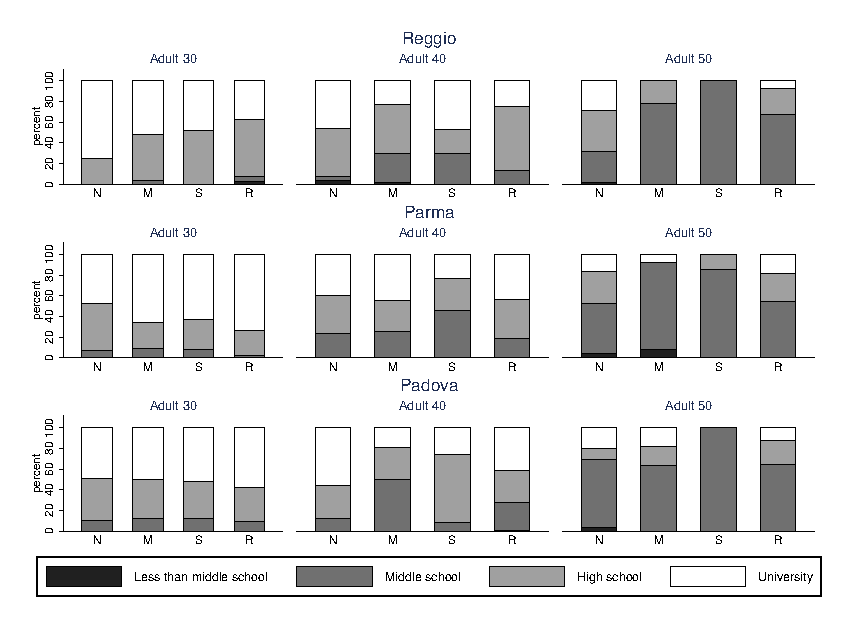
\includegraphics[scale=1.2]{../../Output/image/bar_momEdu}
	\caption{Mother's educational attainment by city, cohort and materna type}
	\label{fig:momEdu}
	\footnotetext{Note:  \textbf{(1)} Definiteion of bar labels: N = Not attended; M = Municipal; S = State; R = Religious. \textbf{(2)} Each bar presents the distribution of mothers' educational attainment for individuals in each city-cohort-materna type combination. }
	\end{minipage}
\end{figure}

\begin{figure}[!htb]
	\begin{minipage}{1\textwidth}
	\centering
	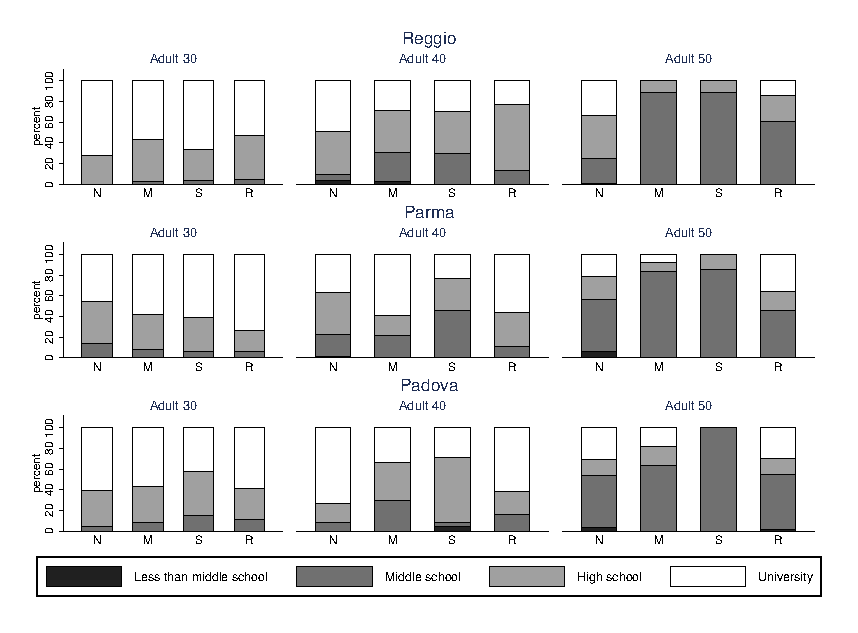
\includegraphics[scale=1.2]{../../Output/image/bar_dadEdu}
	\caption{Father's education attainment by city, cohort and materna type}
	\label{fig:dadEdu}
	\footnotetext{Note:  \textbf{(1)} Definition of bar labels: N = Not attended; M = Municipal; S = State; R = Religious. \textbf{(2)} Each bar presents the distribution of fathers' educational attainment for individuals in each city-cohort-materna type combination. }
	\end{minipage}
\end{figure}

\begin{figure}[!htb]
	\begin{minipage}{.9\textwidth}
	\centering
	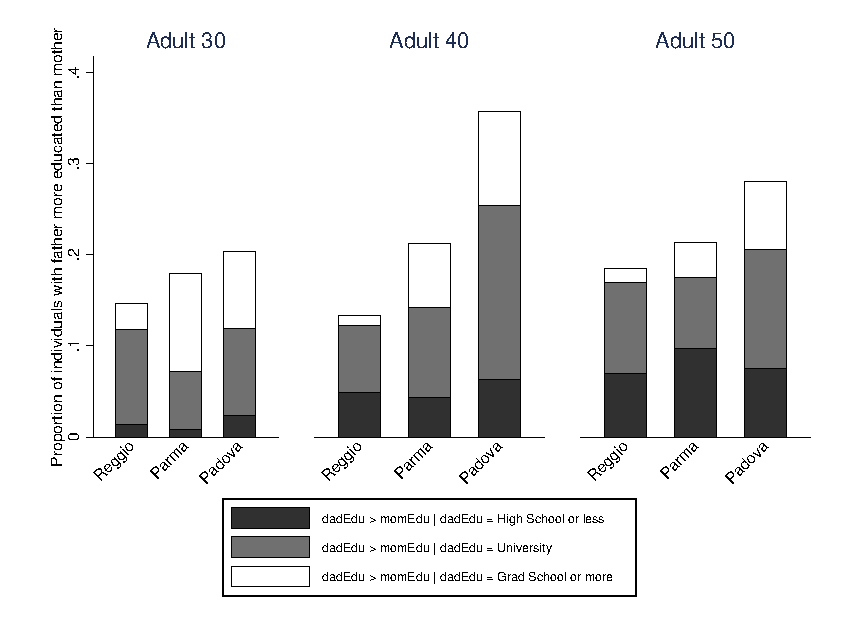
\includegraphics[scale=1]{../../Output/image/bar_parentsEduCompare}
	\caption{Proportion of individuals with fathers who are more educated than mothers by city and cohort}
	\label{fig:parentsEdu}
	\footnotetext{\noindent Note: Each column represents the proportion of individuals within each city-cohort combination whose fathers were more educated than their mothers.}
	\end{minipage}
\end{figure}
